\section{Results}
\label{sec:results}

Tables~\ref{tab:lm} and~\ref{tab:ae} give the 18 declared comparisons, one table per reference, each with the
mean difference and its interval, the median difference, the number of repositories where the model's \qs{}
is lower, the strict win fraction and the adjusted $p$-value side by side. Figure~\ref{fig:paired} shows the
same. The two summaries, the mean and the typical repository, are always shown together because they
disagree.

\begin{table}[t]
\centering\small
\caption{The nine declared comparisons against \lm{}. Differences are model minus reference \qs{}, averaged
over three windows within repository and then over 300 repositories; negative favors the model. The interval
is the pointwise 95 percent percentile interval from 20,000 repository-cluster bootstrap replicates. ``Lower''
counts repositories (of 300) where the model's score is strictly lower; the strict win fraction divides by
300. $p$ is the Benjamini-Hochberg adjusted two-sided Wilcoxon signed-rank $p$-value over the 18 tests.}
\label{tab:lm}
\begin{tabular}{llrcrrrr}
\toprule
Model & $h$ & Mean & 95\% interval & Median & Lower & Win fraction & Adjusted $p$ \\
\midrule
Chronos-2 & 7 & -0.137 & [-0.342, 0.009] & 0.0010 & 79 & 0.263 & $1.0 \times 10^{-5}$ \\
Chronos-2 & 30 & -0.132 & [-0.285, -0.022] & 0.0018 & 59 & 0.197 & $5.5 \times 10^{-12}$ \\
Chronos-2 & 90 & -0.101 & [-0.211, -0.016] & 0.0023 & 50 & 0.167 & $1.4 \times 10^{-13}$ \\
TimesFM 3 & 7 & -0.258 & [-0.718, 0.012] & 0.0003 & 89 & 0.297 & $6.7 \times 10^{-3}$ \\
TimesFM 3 & 30 & -0.201 & [-0.488, -0.024] & 0.0004 & 75 & 0.250 & $8.4 \times 10^{-7}$ \\
TimesFM 3 & 90 & -0.128 & [-0.296, -0.016] & 0.0032 & 54 & 0.180 & $6.4 \times 10^{-12}$ \\
TimesFM 2.5 & 7 & -0.243 & [-0.695, 0.025] & 0.0015 & 68 & 0.227 & $3.2 \times 10^{-8}$ \\
TimesFM 2.5 & 30 & -0.201 & [-0.510, -0.015] & 0.0028 & 49 & 0.163 & $2.4 \times 10^{-13}$ \\
TimesFM 2.5 & 90 & -0.112 & [-0.285, 0.001] & 0.0041 & 46 & 0.153 & $1.9 \times 10^{-14}$ \\
\bottomrule
\end{tabular}
\end{table}

\begin{table}[t]
\centering\small
\caption{The nine declared comparisons against \aets{}, with the same columns as Table~\ref{tab:lm}.}
\label{tab:ae}
\begin{tabular}{llrcrrrr}
\toprule
Model & $h$ & Mean & 95\% interval & Median & Lower & Win fraction & Adjusted $p$ \\
\midrule
Chronos-2 & 7 & -1.069 & [-1.459, -0.700] & -0.1658 & 296 & 0.987 & $2.1 \times 10^{-48}$ \\
Chronos-2 & 30 & -2.127 & [-2.831, -1.536] & -0.2128 & 298 & 0.993 & $3.3 \times 10^{-49}$ \\
Chronos-2 & 90 & -6.724 & [-13.424, -2.868] & -0.2827 & 298 & 0.993 & $3.1 \times 10^{-49}$ \\
TimesFM 3 & 7 & -1.191 & [-1.547, -0.890] & -0.1817 & 297 & 0.990 & $2.2 \times 10^{-49}$ \\
TimesFM 3 & 30 & -2.196 & [-2.915, -1.583] & -0.2171 & 298 & 0.993 & $8.8 \times 10^{-50}$ \\
TimesFM 3 & 90 & -6.751 & [-13.476, -2.871] & -0.2844 & 293 & 0.977 & $1.9 \times 10^{-48}$ \\
TimesFM 2.5 & 7 & -1.175 & [-1.534, -0.874] & -0.1755 & 297 & 0.990 & $2.2 \times 10^{-49}$ \\
TimesFM 2.5 & 30 & -2.195 & [-2.932, -1.580] & -0.2121 & 298 & 0.993 & $8.8 \times 10^{-50}$ \\
TimesFM 2.5 & 90 & -6.735 & [-13.339, -2.871] & -0.2809 & 297 & 0.990 & $3.2 \times 10^{-49}$ \\
\bottomrule
\end{tabular}
\end{table}

\begin{figure}[t]
\centering
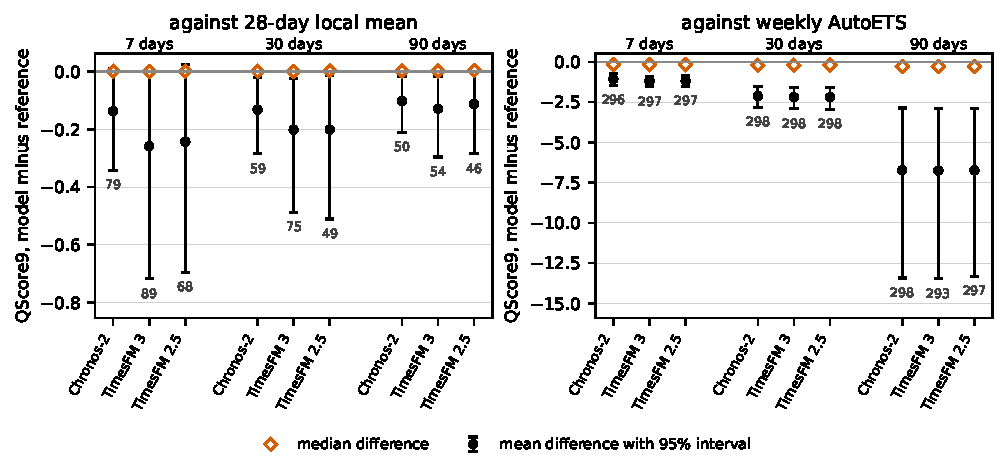
\includegraphics[width=\textwidth]{fig-paired-differences}
\caption{The 18 declared comparisons. Filled circles: mean difference (model minus reference \qs{}) with its
pointwise 95 percent repository-bootstrap interval. Open diamonds: median difference. The number under each
interval is the count of repositories, of 300, where the model's score is lower. Note the different vertical
scales.}
\label{fig:paired}
\end{figure}

\paragraph{Against the local mean.} In all nine cells the mean difference is negative, favoring the model,
from $-0.101$ (Chronos-2, 90 days) to $-0.258$ (TimesFM 3, 7 days), and the bootstrap interval excludes
zero in five cells: the three 30-day cells and the 90-day cells of Chronos-2 and TimesFM 3. The three 7-day
intervals and TimesFM 2.5 at 90 days include zero. In all nine cells the median difference is positive,
favoring the reference, and the model's score is lower on only 46 to 89 of the 300 repositories. The
signed-rank test rejects in all nine cells after adjustment (largest adjusted $p$ 0.0067, TimesFM 3 at 7
days); because every median is positive, the location shift the test detects favors the reference. The
signed-rank test is not a test of the mean, and the bootstrap interval is pointwise, not simultaneous; the
two statements do not contradict each other. The mean is carried by a minority of repositories with large
gains: in the declared scale review the five largest positive repository gains account for 88.5 to 94.3
percent of all positive gain against the local mean, and the leave-one-repository-out mean gain stays
positive in every cell (Appendix Table~\ref{tab:scale}). Ratio skill against the local mean is defined for
only 209, 239 and 259 of 300 repositories at 7, 30 and 90 days, because the reference's loss is zero on the
others; the report does not headline a ratio.

\paragraph{Against AutoETS.} In all nine cells both the mean and the median difference are negative, the
model's score is lower on 293 to 298 of 300 repositories, and the signed-rank test rejects in all nine; both
summaries favor the model. Mean differences grow with horizon, from $-1.07$ to $-1.19$ at 7 days to $-6.72$
to $-6.75$ at 90 days, and the 90-day intervals are wide. The reason is in the reference: AutoETS's nominal
80 percent intervals cover 98.6 to 98.8 percent of target days pooled over the panel (a declared secondary
summary), and in a width diagnostic requested after the run within that declared analysis its median 90-day
daily interval width is 0.79 stars per day in the smallest stratum, 3.60 in the middle one and 49.69 in the
top one (Appendix Table~\ref{tab:autoets}). Six fits at each horizon, from two repositories, selected
multiplicative seasonality, all in the top stratum; the specification counts were also requested after the
run. AutoETS is a weak uncertainty reference on this panel.

\paragraph{By stratum and calibration.} Pooled \qs{} by stratum (Appendix Table~\ref{tab:stratum}) holds
stratum means only: in the top stratum the three models' pooled scores are below the local mean's at every
horizon; in the smallest stratum the local mean's is below all three at every horizon; in the middle stratum
the four differ by less than 0.012 at every horizon; and AutoETS is far above all of them at every scale. The
typical repository by stratum is not in the declared tables. A post-hoc reading of the saved per-repository
accounting file, which adds no test, gives it: the median difference against the local mean is positive,
favoring the reference, in every stratum and every cell, and the models score lower on 5 to 18 of 100
repositories in the smallest stratum, 10 to 34 in the middle one and 26 to 38 in the top one. So the stratum
means and the typical repository disagree within the top stratum as the panel mean and the typical repository
disagree overall. Inclusive 80 percent coverage of the repaired deciles over the panel is 0.824 to 0.837 for
Chronos-2, 0.880 to 0.910 for TimesFM 3, 0.906 to 0.924 for TimesFM 2.5, 0.941 to 0.955 for the local mean
and 0.986 to 0.988 for AutoETS (Appendix Table~\ref{tab:calibration}). On discrete counts a correct quantile
can overcover \citep{czado2009}, so these are descriptive.
